\documentclass{report}
\usepackage{graphicx}
\usepackage{listings}
\usepackage{amsmath}
\usepackage[pict2e]{struktex}
\usepackage{parcolumns}
% \usepackage{multicol}
%\usepackage[rflt]{floatflt}

%\usepackage{fullpage}

%I've found the following lines in the internet to automatically begin a new line after a paragraph
\makeatletter
\renewcommand\paragraph{\@startsection{paragraph}{4}{\z@}%
  {-3.25ex\@plus -1ex \@minus -.2ex}%
  {1.5ex \@plus .2ex}%
  {\normalfont\normalsize\bfseries}}
\makeatother

%to change section numbering depth to 3 (default 2)
\setcounter{secnumdepth}{3}

%to change depth for appearence in table of contents to 3 (default 2)
\setcounter{tocdepth}{3}

\begin{document}

% \documentclass[12pt]{article}

% \usepackage{ngerman}
% \selectlanguage{ngerman}
% \usepackage[latin1]{inputenc}

% \usepackage{graphicx}

% \begin{document}

\pagestyle{empty}

\begin{center}

\vspace*{-2.8cm}
\begin{minipage}[c]{.30\textwidth}
  \begin{flushleft}
    \includegraphics[width=3cm,clip=]{LOGO/new-aerlogo.eps}%
  \end{flushleft}
\end{minipage}
\begin{minipage}[c]{.43\textwidth}
    { ~\\ Lehrstuhl f\"{u}r Aerodynamik \\ Prof.~Dr.-Ing. N.~A.~Adams}%
\end{minipage}
\begin{minipage}[c]{.25\textwidth}
  \begin{flushright}
    \vspace*{1em}
    
\includegraphics[width=3cm,clip=]{LOGO/TUMLogo_oZ_Vollfl_blau_RGB.eps}%
  \end{flushright}
\end{minipage}

\vspace*{3.3cm}
\begin{minipage}[c]{11cm}
{\LARGE\bf 
A Riemann solver }
\end{minipage}

\vspace*{0.8cm}
Mark F\"{o}rster\\

\vspace*{2.8cm}
{\bfseries Diplomarbeit}

\vspace*{1.2cm}
%\large
\normalsize
\vfill
\begin{tabular}{ll}
Betreuer: &  Dr.-Ing. Christian Stemmer \\
\ & \ \\
Ausgabe: & 1.\ Oktober 2008\\
Abgabe: & 31.\ M\"{a}rz 2009\\
\end{tabular}

\vspace*{1.6cm}
%\large
Lehrstuhl f\"{u}r Aerodynamik an der Technischen Universit\"{a}t M\"{u}nchen\\
2009
\end{center}

\pagebreak
\pagestyle{plain}

%\end{document}



\tableofcontents
\chapter{Introduction}
\label{sec:intro}


This work aimes at the numerical simluation of high enthalpy flow in
porosities. The subject is of interest, as CITATION
NEEDED (Prof Hornung) has discovered porous surfaces to inhibit/block a
certain form of instabilities in hypersonic flows over a body/cone. A numerical
simulation of this configuration is desired to furnish data for a detailed
analysis of the acting phenomena. The simulation method of choice for the first approach
to this configuration is called Smoothed Particle Hydrodynamics (SPH). Although
there has been no known application of SPH to this precise/concrete case yet/before,
SPH is adopted, as it promises a crucial advantage in the way boundary
conditions are implemented. And for the treatment of porosities,
boundaries/walls represent a non negligible part of the problem.

SPH designates a meshfree method for numerical simulation of particle
ensembles (respectively matter that can be modelled as an ensemble of
particles as it is the case for fluids).
Thereby,the term particle ensembles not only refers
to fluids (as the name of the method would suggest) but also to solids. In
fact nowadays SPH is employed to simulate problems in different fields,
such as body elasticity and fracture,liquid flows and gas
dynamics~\cite{Monaghan2005}.
The initial developement of the method dates back to 1977, where Gingold and
Monaghan tempted to compute an astrophysical gas dynamics problem with a new, more
efficient method~\cite{Gingold1977}. Independently and simultaneously, work in
this field was also carried out by Lucy who came up with the same
idea~\cite{Lucy1977}.
ADVANTAGES???DISADVANTAGES???

PREVIOUS APPLICATIONS IN GAS DYNAMICS (citing different relevant papers)

OTHER APPROACHES FOR CAVITY/POROSITY SIMULATION (look up in literature)

INTRODUCE THE TWO CODES AND MENTION THAT THEY ARE CODED IN C/C++...



\chapter{Method}
\label{sec:method}
\section{Basic Idea of SPH}
\label{sec:BasicsSPH}

To illustrate the basic idea of SPH, it is helpful to first have a look at the
ruling equations of fluid dynamics, here represented by the Navier stokes equations in
lagrangian form (using the substantive derivative). The use of the lagrangian form seems logical as SPH is a
particle method.

\begin {equation}
NAVIER STOKES IN LAGRANGIAN FORM
\end {equation}

The above equations have the form~\cite{Monaghan2005}

\begin {equation}
\label{eq:EFD_form}
{\frac{dA(r)}{dt}}=f(A(r),\nabla A(r),r)
\end {equation}
where
\begin {equation}
{\frac{d(.)}{dt}}={\frac{\partial(.)}{ \partial t}}+v\nabla(.)
\end{equation}
is the substantive derivative.

Thus the rates of change of  physical quantity depend on its spatial
derivatives. The goal of any method for numerical simulation is to approximate
these derivatives by information of a discrete number of points in order for a
computer to be able to handle it. 


The SPH method is based on the idea of approximating a function $A(x)$ by an
integral interpolant
\begin{equation}
\label{eq:int_interpolant}
A_I(x)=\int A(r')W(r-r',h)dr'
\end{equation}
where $W(r-r',h)$ is the so called kernel or smoothing function and $h$ the
smoothing length. This Interpolation is exact, if $W$ is the delta function,
otherwise it describes/represents an approximation. As the theoretically
perfect Kernel, the delta function, is of no practical use, the Kernels
employed in practice are functions which tend to the delta function, when $h$
tends to zero. Examples for those kernel functions are a Gaussian Kernel or
Kernels based on Schoenbergs~\cite{Schoenberg1946} $M_n$ splines~\cite{Monaghan2005}. More details on Kernels are given in the section
(LINK TO SECTION??) and in the book on SPH published by Liu~\cite{Liu2003}

The fact of using a kernel different from the delta function constitutes/is the
first of two approximations /approximative assumptions made for the SPH
method. It is often refered to as kernel approximation~\cite{Liu2003}.
The second approximation consists of a discretization of the integral
expression in equation\ref{eq:int_interpolant}, leading to a summation over
all discretized elements (the particles) of the domain instead
of an integration when calculating the interpolant value $A_I(x)$, which
finally allows a treatment of the problem by a numerical machine. In SPH
literature, this second approximation is commonly called particle
approximation~\cite{Liu2003}

With the relation between mass, density and volume for each discretized particle
\begin{equation}
m_i=\rho_i V_i
\end{equation},
applying the particle approximation on \ref{eq:int_interpolant} leads to the following expression

\begin{equation}
\label{eq:intInter}
A_S(r)=\sum_b m_b \frac{A_b}{\rho_b}W(r-r_b,h)
\end{equation}


In the same way, the derivative of the field function $frac{dA(x)}{dx}$ can be
approximated to give\cite{Monaghan2005}or\cite{Liu2003}(in Liu with gradient,
im Monaghan for 1 direction)

\begin{equation}
\label{eq:simpleDerivative}
\nabla A_S(r)=\sum_b m_b \frac{A_b}{\rho_b}\nabla W(r-r_b,h)
\end{equation}

The disadvantage of the above equation \ref{eq:simpleDerivative} is, that for
$A(r)=const.$ the approximated derivative does not vanish. By writing (in
Monaghan the equation figures not with gradient but only in 1 direction!?!)
\begin{equation}
\label{eq:derivativeIdentity}
\nabla A = \frac{1}{\Phi}(\nabla {\Phi A}-A\nabla \Phi)
\end{equation}
where $\Phi$ is any differentiable function, this problem can be resolved. In its
SPH form  equation \ref{eq:derivativeIdentity} reads as follows:

\begin{equation}
\nabla_a A = \frac{1}{\Phi_a}\sum_b \frac{m_b}{\rho_b}(A_b-A_a)\nabla_a W_{ab}
\end{equation}


It can be seen, that the (approximation of the) derivative of the
field function $A$ is now expressed by a summation over the field function itself
and the derivative of the kernel function - which can be determined exactly.

Now the basic formulations are introduced in principle: Both the fieldfunction
itself and its spacial derivatives can be approximated using only information of a discrete number of particles. Hence, the change rates of
the states described by the equations of fluid dynamics, which have a form
according to \ref{eq:EFD_form} can be rewritten using this information. Doing
this one obtains the SPH formulation of the equations of fluid dynamics.

The detailed derivation of those equations will not be shown here, as the
interest  only lies in describing the principle ideas behind the SPH
method. To resume, this are the following ones: A (field) function can be
described as an integral interpolation over the function itself and a kernel
function (which has to be chosen in an appropriate way). A further
approximation consists in transforming the integral over the domain into a
summation over the discrete elements constituing this domain (the particles). This allows to express both
the field function and its spacial derivatives dependent exclusively on discrete values
of the fieldfunction itself (and of the kernel function, which is known as well as
its derivatvies). By finally choosing an appropriate kernel function with
compact support, the summation over all particles in the domain can be reduced
to a summation over those particles within the support domain of the particle
in question.

As already mentionned above, the SPH formulation of the equations of fluid
dynamics is obtained by applying the above principles and conducting different
transformations to the original (exact) equations. Depending on the
transformations used, the final SPH equations can assume a different form. In
the following, a common form for the change rates of density, velocity and
internal energy based on the EULER EQUATIONS (i.e. without viscosity) is
listed\cite{Monaghan2005,Liu2003} (perhaps also list NSG-form, and
explain why Euler is of interest as well (for 1DSPH code, perhaps later real
code including viscosity???)

\begin{equation}
\label{eq:DCR_Euler}
\frac{d\rho _a}{\mathit{dt}}=\sum{m_{b}v_{\mathit{ab}}\nabla _{a}W_{\mathit{ab}}}
\end{equation}

\begin{equation}
\label{eq:VCR_Euler}
\frac{dv_{a}}{\mathit{dt}}=-\sum {m_{b}\left(\frac{P_{a}}{\rho_{a}^{2}}+\frac{P_{b}}{\rho _{b}^{2}}\right)\nabla_{a}W_{ab}}
\end{equation}


\begin{equation}
\label{eq:ECR_Euler}
\frac{de_{a}}{\mathit{dt}}=-\mathit{}\frac{1}{2}\sum{m_{b}\left(\frac{P_{a}}{\rho _{a}^{2}}+\frac{P_{b}}{\rho _{b}^{2}}\right)v_{\mathit{ab}}\nabla _{a}W_{\mathit{ab}}}
\end{equation}

For the detailed procedure of derivation and for alternative formulations of
these equations refer to \cite{Monaghan2005, Liu2003}

Artificial Viscosity

(perhaps I will move this section and make it a subsection of 'Implementation of SPH' (as artificial viscosity is linked to numerics

Another point that has to be taken into account for SPH simulations, especially
such including shock phenomena, is arificial viscosity\cite{Monaghan2005}. It
prevents particles from penetrating one into an other in zones with high
compression rates and also generally stabilizes a numerical
allgorithm.
Artificial viscosity for numerical simulation of shock phenomena
in general was first introduced by \cite{vonNeumann1950}. They suggested to
introduce an artificial dissipation to give the shock a thickness which
allowed it to be calculated numerically (in the cited example with finite difference
scheme) without introduction of pre-/after shock boundary conditions.    ...(see article)
The first use of artificial viscosity specifically for the mesh free SPH goes
back to Lucy\cite{Lucy1977}. He suggested an artificial bulk viscosity to
prevent a slow buildup of acoustic energy by integration errors in zones with
low density respectively low particle presence. 
Finally, the form of artificial viscosity most commomly used in SPH
literature\cite{Liu2003} is the one proposed by Monaghan and
Gingold\cite{Monaghan1983}. They stated that the use of one of the artificial
viscosities cited above (Neumann Richtmyer (adapted to SPH) or bulk
viscosity) on shock problems would lead to either excessive particle
oscillation or excessive smearing of the shock front. The expression for this
artificial viscosity $\Pi_{ab}$, which is added to the pressure term of
equation \ref{eq:VCR_Euler}, is:

\begin{equation}
\label{eq:MonArtVis}
\Pi _{\mathit{ab}}=-\nu
\left(\frac{v_{\mathit{ab}}r_{\mathit{ab}}}{r_{\mathit{ab}}^{2}+\epsilon
h_{\mathit{ab}}^{2}}\right)
\end{equation}
where 
\begin{equation}
\label{eq:FactArtVis}
\nu =\frac{h_{\mathit{ab}}}{\rho _{\mathit{ab}}}\left(\alpha
c_{\mathit{ab}}-\beta
\frac{h_{\mathit{ab}}v_{\mathit{ab}}r_{\mathit{ab}}}{r_{\mathit{ab}}^{2}+\epsilon
h_{\mathit{ab}}^{2}}\right)
\end{equation}

$v_{ab}$ stands for $v_a-v_b$, $r_{ab}$ for $r_a-r_b$, $c_{ab}$ is the
averaged sound speed of the two particles in question $1/2(c_a+c_b)$. The same
applies for $\rho_{ab}(=1/2(\rho_a+\rho_b))$ and $h_{ab}=(1/2(h_a+h_b))$. IT
HAS TO BE MENTIONED SOMEWHERE (but probably not right here) THAT: the use of
the averaged smoothing length $h_{ab}$ is a way to symmetrize particle
interactions when h is spatially variable. In this case a particle $a$ could be
located in the support domain of a particle $b$ but not vice versa. This would
lead to an assymetric mutual contribution of forces. To avoid this, using the
averaged smoothing length between two particles is an appropriate remedy\cite{Liu2003}.
Including artificial viscosity, the SPH form of the Euler momentum equation becomes\cite{Monaghan2005}

\begin{equation}
\label{eq:VCR_EulerInclArtVis}
\frac{dv_{a}}{\mathit{dt}}=-\sum {m_{b}\left(\frac{P_{a}}{\rho_{a}^{2}}+\frac{P_{b}}{\rho _{b}^{2}}+\Pi _{ab}\right)\nabla_{a}W_{ab}}
\end{equation}

The introduced artificial viscosity must also be reflected in the energy equation, as viscosity transfers energy from kinetic to thermal\cite{Monaghan2005}. One formulation of the energy equation which is convenient for implementation in the 1D SPH code (as a big part of the needed expression has already been calculated for \ref{eq:VCR_EulerInclArtVis}) can be found in\cite{Liu2003}

\begin{equation}
\label{eq:ECR_EulerInclArtVis}
\frac{de_{a}}{\mathit{dt}}=-\mathit{}\frac{1}{2}\sum{m_{b}\left(\frac{P_{a}}{\rho _{a}^{2}}+\frac{P_{b}}{\rho _{b}^{2}}\right)v_{\mathit{ab}}\nabla _{a}W_{\mathit{ab}}}
\end{equation}

...mention somewhere that kernel unity is inverse of volume?!?!?

\section{Implementation of an SPH code}
This section presents some particular features of an SPH code. Emphasis is
placed on these features which are finally implemented in one of the
two SPH codes designed and modified during this work.
Points of interest are the implementation of different boundary conditions in
SPH, a closer description of the kernel function, as well as different methods/allgorithms
to perform the search for the interacting particles. Furthermore different
equations of state are introduced, depending on the nature of the flow problem
to be considered(compressible/incompressible). Finally some words on numerical
integration schemes that have proven to be reliable for SPH applications.


\subsection{boundary condition implementation}
\label{sec:boundaryConditionImplementation}
For particles at the edge of the calculation domain, the summation interpolation does not
give exact results, as the integral (or better the sum) is truncated due to
the simple fact that outside the domain there are no
particles.\cite{Liu2003}(find better citation...) This efect is called the
problem of article deficiencythe particle deficiency
problem.\cite{Liu2003}. In some cases there is no need to consider this
problem, as the areas close to the edges are not of interest and due to
limited simulation time there is no time for the error to propagate into the
actual zone of interest. The 1D shock tube simulation described further below
(PERHAPS LINK TO SECTION)is an example for such a case.  
But for other applications the edges play an important role or the domain has
to be rendered periodocally. So there is a need to define specific boundary
conditions. This can be accomplished by a special boundary treatment, which
often includes so called virtual particles or ghost
particles\cite{Liu2003}. The first ones to come up with this idea were
\cite{LIBERSKY1993}. Virtual particles are used to model solid walls by
placing them inside the solid body, mirrored at the surface. For each real
particle whose support domain interfres with the wall, one such particle is
built. Virtual particles have the same properties as their real counterpart
except for the velocity. Depending on the type of boundary condition they are
supposed to represent, different velocities are assigned to them.\cite{Hu2006}

non slip velocity boundary condition

\begin{equation}
v_{virtual}=2v_{wall}-v_{real}
\end{equation}

free slip velocity boundary condition

\begin{equation}
v_{virtual}^{tangential}=v_{real}^{tangential}
\end{equation}

FIGURE: ILLUSTRATION OF VELOCITY ASSIGNMENT FOR VIRTUAL BOUNDARY PARTICLES

For the treatment of periodic boundary conditions, no ghost particles are
needed. Particles leaving the calculation domain on one side are simple
reinserted on the opposite side (with the same properties).


\subsection{kernel function}
\label{sec:KernelFunction}
???not sure, if its the right place here, but somewhere there should be a
paragraph with more detailed information on kernels used, compact support,
perhaps even some properties,...(and perhaps some graphics???)


Some properties of Kernel functions (smoothing functions) and notions related
to them have allready been mentionned in the section
\ref{sec:BasicsSPH}. In principal every function can act as Kernel function
when it respects a set of criteria complsed by \cite{Liu2003}.
The most important ones are:

The smoothing function should vanish outside of a certain area around its
center. This property is called compact support and the domain where $W\neq0$
the support domain of the smoothing function. The smoothing length $\kappa h$ and the
support length $h$ may not be mixed up.
\begin{equation}
W(x-x')=0,\textit{for}|x-x'|>\kappa h
\end{equation}

The smoothing function should be normalized to 1, which ensures that constants
are interpolated exactly
\begin{equation}
\int{W(x-x',h)dx'}=1
\end{equation}

The smoothing function should tend towards the delta function as/when the smoothing
length $h$ tends to zero
\begin{equation}
\lim\limits_{h \rightarrow 0}{W(x-x',h)}=\delta(x-x')
\end{equation}
This is to ensure consistency of the integral approximation, which means that
the approximative expression tends to the exact expression of the integral
interpolant equation.

The full list of SPH kernel properties can be found in  \cite{Liu2003}.
Based on those properties a variety of Kernels are used in SPH literature. A
very commonly used Kernel though is the $M_4$ Kernel (Cubic Spline) based on Schoenbergs
$M_n$-Splines\cite{Schoenberg1946}.

\begin{equation}
\label{eq:cubicSpline}
M_{4}(x)=\begin{cases}
\frac{1}{6}[(2-q)^{3}-4(1-q)^{3}],& \text{for 0 $\leq$ q $\leq$ 1} \\
\frac{1}{6}(2-q)^{3},&  \text{for 1 $\leq$ q $\leq$ 2} \\
O,& \text{for q $>$ 2}
\end{cases}
\end{equation}


In the work of \cite{Fulk1996} a mesure of merit for Kernels is developed and
they came to the result, that in 1D no kernel performed significantly better
than the cubic spline.
This is why for the 1D SPH code described in section (WHATEVER) the cubic
spline kernel is employed.

\subsection{neighboring particle search methods}
\label{sec:NNPS}
To calculate the change rates in \ref{eq:DCR_Euler}-\ref{eq:ECR_Euler} a
summation over all paricles has to be performed. However, as we defined kernel
functions with a compact support, only particles within a certain distance from
the particle in question (within its support domain) contribute to the
interpolation of its values, and thus interact. Finding the interacting
particles is one of the key features in an SPH implementation, as an effective
interaction search method (often also called nearest neighboring particle (NNP)
search method in SPH literature) can considerably speed up/accelerate
computation time. 

The most basic NNP algorithm is called all pair search, and as its name
suggests all imaginable particle pairs are tested for interaction. This means
the calculation process consists of a double loop where the outer loop
iterates over all particles and defines one of the pair's partners (often
refered to as origin). For each of the (origin) particles an inner loop is
performed, which iterates again over all particles thus defining the oterh
partner (destination) of the pair. Then, the pair is tested for the
interaction condition, meaning that their distance has to be inferior to the
support length. In this way, for a calculation domain consisting of $N$
particles, $N*N$ iteration steps and tests have to be executed. The
calculation cost of this approach is of the order $O(N^2)$. 
If the
interactions are assumed pairwise (i.e. if there is a spacially constant
smoothing (and therefore support) length; THINK ABOUT THE AVERAGED SMOOTHING
LENGTH...) there is a simple but efficient way of reducing computation
time. In this case namely, if the pair $P_{ij}$ is an interaction, the pair
$P_{ji}$ is an interaction as well. That way half of the $O(N^2)$ iterations
and tests can be avoided leading to a complexity of $O(N!)$ (LOOK FOR
REFERENCES). This approach is employed in the 1D SPH code as it is easy to
implement\cite{Liu2003} and the number of particles in this 1D simulation is
still reasonably low in order not to have to use more sophisticated algorithms
like they are introduced below.

A more effective but also more complicated method is the linked list
algorithm. Its idea is based on the fact, that kernels wit compact suport are
used and thus interacting particles may only be located in the neighborhood of
the considered particle. The computation domain is divided into cells (with
cell size$\ge \kappa h$, ideally $=\kappa h$) and the
particles are assigned to the cell they are located inc\cite{Monaghan1983}. In this way the cell
structure serves as a book keeping device and in case of an interaction
calculation with an origin particle $i$ not all the particles $j,j={1,...,N}$ have
to be considered but only those particles in the adjoining cells. Hence, the
complexity of the original problem which is of order $O(N^2)$ can be reduced
largely and tends even to $O(N)$ if the particles in one cell are few. 

FIGURE: DIAGRAM WITH CELLS /PARTICLES /DOMAIN!?!

Technically the cells are managed by the implementation of a linked list
structure in a computational code. More details on this are given in section
(SOMEWHERE IN 2D CODE DESCRIPTION), as this algorithm is implemented in the 2D
SPH code, and in \cite{Monaghan1985, Hockney1988}.
The method however has a drawback if used with a spacially variable smoothing
length. In this case the cell size is not ideally adapted to every particle
and the allgorithm looses efficiency.

Moreover, different other NPP techniques exist which, here, shall not be introduced in
detail. One of them are tree search algorithms\cite{Hernquist1989}, which are
especially robust and efficient for problems with variabe smoothing
length\cite{Liu2003}.



\subsection{equation of state}


The equation of state allows for the computation of the pressure $p$ based on
information about the density $\rho$ and the internal energy $e$ (or equivalent...). For the application of SPH for gas dynamics, the assumption of an ideal gas is appropriate (citation and conditions). In this case the (ideal gas) equation of state is

%...equation of state in the original form...

%...
%transformation steps (or at least realations needed)...

\begin{equation}
 p=(\gamma-1)\rho e
\end{equation}

The sound speed, which is needed to calculate the artificial viscisoty (see (\ref{eq:FactArtVis})), can be formulated for an ideal gas as:

\begin{equation}
 c=\sqrt{\gamma R T}
\end{equation}
or with $c_v T=e$, $R=c_p-c_v$ and $\gamma=\frac{c_p}{c_v}$

\begin{equation}
 c=\sqrt{\gamma(\gamma-1)e}
\end{equation}


???shold I mention the equation of state applied for liquids (by artificially
introducing a little compressibility \cite{Monaghan1994,Monaghan2005}???




\subsection{numerical integration}
\label{sec:numIntegr}

As far as the time integation of the equations of SPH is concerned, any stable
time stepping algorithm for ordinary differential equations may be
used\cite{Monaghan2005}. However for SPH simulations, the conservation properties
(linear and angular momentum) of the integrator are more important than its
order\cite{Monaghan2005}.

Thus, a stadard leap frog scheme is one possibility to perform the integration in
time. The initial time step is done according to the following algorithm where
$S$ is a substtitute for $\rho,v,e$

For $n=0$:
\begin{equation}
S_{\frac{1}{2}}=S_0+\frac{1}{2}dt\left(\frac{dS}{dt}\right)_0
\end{equation}
\begin{equation}
x_1=x_0+dt v_{\frac{1}{2}}
\end{equation}

for any further time step $n\ge1$:

\begin{equation}
S_n=S_{n-\frac{1}{2}}+\frac{1}{2}dt\left(\frac{dS}{dt}\right)_{n-1} \rightarrow
\frac{dS}{dt})_n 
\end{equation}
\begin{equation}
S_{n+\frac{1}{2}}=S_{n-\frac{1}{2}}+dt\left(\frac{dS}{dt}\right)_n 
\end{equation}
\begin{equation}
x_1=x_0+dt v_{\frac{1}{2}}
\end{equation}

Another possibility for time integration is a predictor corrector scheme, as
used by \cite{Hu2007}(IS THIS REFERENCE OK?). The 2D SPH code structure being based on their work,
this integration scheme is implemented in the above mentionned program.

In the predictor step a guess $\hat S$ of the value $s$ at $n+1$ is made by simply
applying a normal Euler step.

\begin{equation}
\hat S_{n+1}=S_n+dt\left(\frac{dS}{dt}\right)_n
\end{equation}
\begin{equation}
x_{n+1}=x_n+dt v_{n}
\end{equation}

This guess is then corrected by a central scheme to update the values at
$n+1$:

\begin{equation}
S_{n+1}=S_n+dt\left(\frac{dS}{dt}\right)_{n+\frac{1}{2}}
\end{equation}

The values at $n+\frac{1}{2}$ needed to calculate
$\frac{dS}{dt})_{n+\frac{1}{2}}$ are obtained by taking the mean value of
$S_n$ and $\hat S_{n+1}$:

\begin{equation}
S_{n+\frac{1}{2}}=\frac{1}{2}(S_n+\hat S_{n+1})
\end{equation}

\subsection{Summation Density and Continuity Density approach}
\label{sec:DensCalcMode}
One way to update/calculate the density with the SPH method is simply to integrate the density change rate \ref{eq:DCR_Euler} for each time step, just like it is done for velocity and internal energy. Thanks to the character of the SPH formulation, there is another possibility of obtaining density. Taking the interpolation equation \ref{eq:intInter} and supposing $A$ is the density $\rho$ gives an expression for the interpolation (the smoothing) of the density of a particle $a$ by summing over all particles within the support domain\cite{Monaghan2005}.

\begin{equation}
\label{eq:SumDensity}
\rho(r)=\sum_b m_b W(r-r_b,h)
\end{equation}

The first method where density is integrated using \ref{eq:DCR_Euler} is refered to as continuity density approach, the second one where density is obtained by summation/smoothing as summation density approach \cite{Liu2003}. Both methods are commonly used in SPH codes, they are often even implemented both in one same code. ADVANTAGES/DISADVANTAGES SEE LIU AND REFERENCES...

\subsection{basic structure of an SPH code}

Any implementation of an SPH code possesses a certain basic structure defined by the nature of the SPH equations. \ref{fig:BasicSphCode} (adapted from \cite{Liu2003}) together with the description in this paragraph shall show the interdependence of the constituent parts of an SPH code in principle. The actual (control) flow of an implememented SPH code may differ in details from \ref{fig:BasicSphCode} and can be seen on/from the more detailed flow diagrams for the specific codes.
Remark: the structure described in the following paragraph applies to any (serial, not parallel) SPH code (no matter if compressible/incompressible or viscous/inviscous). The equations referred to however, are the SPH form of the Euler equations and thus are only valid for invscid problems.

\ref{fig:BasicSphCode} shows that the first essential part of an SPH program is the setting up of the initial conditions includuing the definition of geometrical and other probem specific parameters. The choice of the variables/quantities given as initial conditions not being unique, there are several possibilities in defining them. (for example giving $m$ and $\rho$ defines the particle spacing (which corresponds to the volume) and giving the spacing and $\rho$ fixes $m$.) Which way is selected for a specific program is precised in the corresonding section. 
Thereafter the program enters the main computation loop and the operations executed therein are repeated for each time step. Among those operations is the creation of the virtual boundary particles (\ref{sec:boundaryConditionImplementation}) which are then needed included in the nearest neighbouring particle search (\ref{sec:NNPS}). After having determined all the interactions for all particles the smoothing function and its derivative can be computed for each interaction pair. Then, depending on the density calculation mode (?see? \ref{sec:DensCalcMode}), the program sequence differs slightly. 
For/with the summation density approach, density is obtained by summation (smoothing)\ref{eq:SumDensity} and once density is calculated, the forces on the particles may be determined. Those forces allow for the computation of the momentum change rate (remark: the calculation of forces and momentum change rate can be considered as one single step, all included in \ref{eq:VCR_Euler}). Also, the energy change rate is determined \ref{eq:ECR_Euler}.
As for the continuity density approach, the calculation of forces is conducted without smoothing, taking the density value obtained at the previous step (or the initial value for the first time step). But the density change rate has to be determined as well \ref{eq:DCR_Euler}, as density will be obtained by integration. 
Once all necessary change rates are known, the values can be updated to the next time step, see \ref{sec:numIntegr} and the loop can be restarted. After the actual simulation is finished, an output module is in charge of making data available in a form (that is) exploitable to the user.


\begin{figure}[h]
  \centering
     % 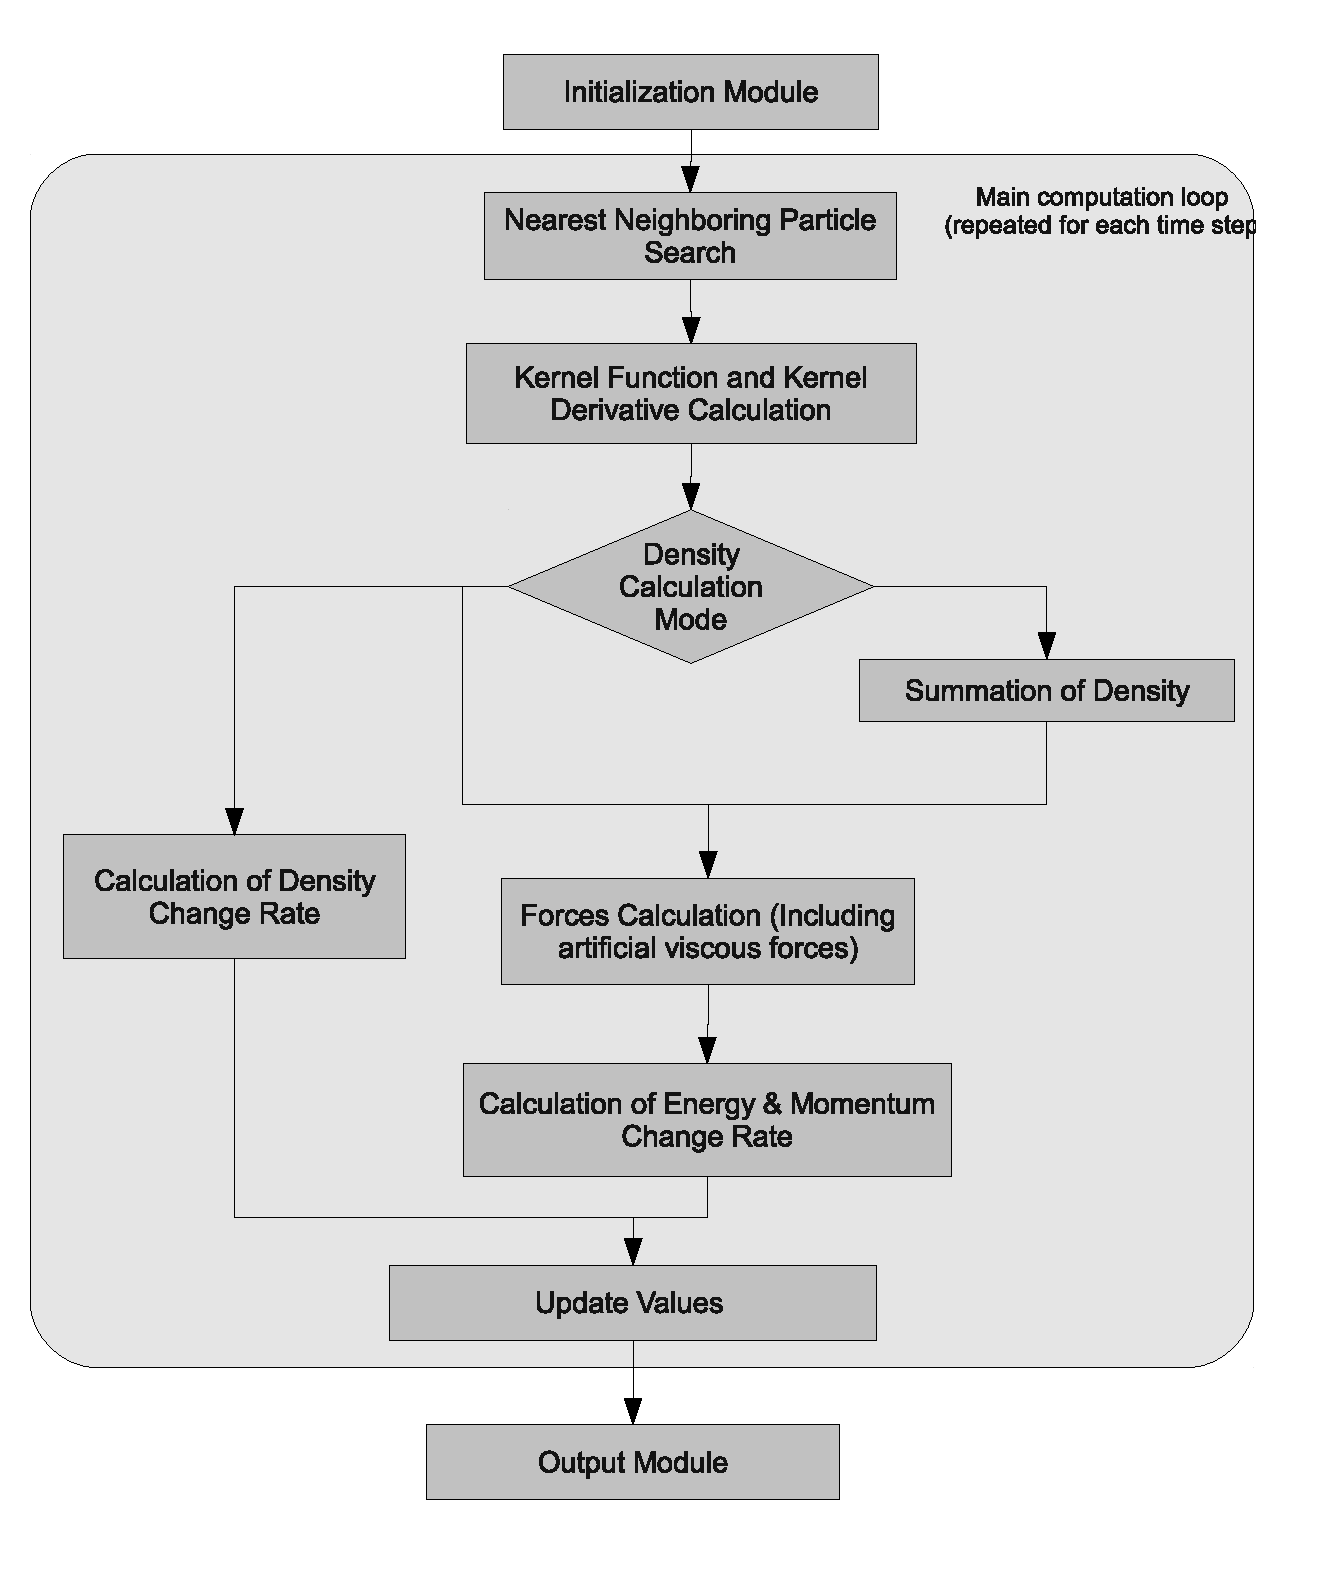
\includegraphics[width=1.0\textwidth]{Graphics/general_structure_SPH}
  \caption{basic structure of an SPH code}
  \label{fig:BasicSphCode}
\end{figure}

\section{1D SPH code}

\subsection{short overview}
PERHAPS THIS SUBSECTION TITLE IS REMOVED AND THE FOLLOWING TEXT WILL FIGURE JUST BELOW THE SECTION TITLE!?!

This code has a relatively simple structure, yet it features all the components a more sophisticated SPH computational program would incorporate. Both the summation density approach and the continuity density approach are implemented \ref{sec:DensCalcMode} By computing a 1D shock tube problem, the code is used to verify the basic SPH equations which are then implemented in the more complex 2D program. As the analytical solution for this problem is well known, the shock tube is a very common test case for 1D compressible codes \cite{Sod1978} (PERHAPS ONE MORE REFERENCE WHICH STATES THAT SHOCK TUBE IS A COMMONLY USED TEST CASE...). The problem setup and the obtained results are discussed in the corresponding section.

\subsection{Validation Case}
As mentionned above, the test case for this 1D compressible SPH code is a 1D shock tube problem. It is introduced already at this stage as it is referred to sometimes in the following section.
In general a shock tube consists of two initially separated (e.g. by a diaphragm) gas filled areas, one side under higher pressure than the other....

PLUS FIGURE SHOCK TUBE

\subsection{components and structure}


\subsubsection{the data structures}

To facilitate the implementation and the handling of the code, two data structures (have been) are defined. 

\paragraph{The parameters data structure}

This data structure is defined in the header file parameters.h(WRITE IN CODE STYLE) and containes all parameters needed to set up the problem. Among those parameters are geometrical values, the initial conditions,simulation length and time step (IN AN EARLY VERSION; IN A LATER VERSION TRY TO ADAPT TIME STEP AUTOMATICALLY!!!!?!!!) as well as parameters defining the fluid properties.

\paragraph{The simulation data structure}

Defined in the file simulation.h(WRITE IN CODE STYLE) this structure is made up of all variables that change in the course of the simulation. To begin with, these are the values of interest like position, velocity, density, pressure, energy, etc.. Furthermore there are variables needed as intermediate results (such as the smoothing length and its derivative). 
Most of the variables contained in the simulation data structure are needed one per particle. Therefore those variables are defined as vectors with a size that corresponds to the number of particles in the system. 

\subsubsection{The Functions}

As the size of the 1D SPH program is not too big, it admits of the introduction/description of every single function used. The textual description is not complete but only comprises particularities and features that are considered worth mentionning. A Nassi-Schneidermann-Diagram (NSD)~\cite{Nassi1973} complements each description and shows the control flow for each function as well as the interdependence of the individual functions. For the sake of a clear illustration , the NSD does not display every loop of the program; frequently, loops over all particles and the interaction list are ommitted (the instruction 'calculate ... for each particle' for example means the implementation of a loop over all particles i.e. all components of the corresponding variable's vector).  Consulting the comments in the source code is recommended if an even more detailed understanding is necessary or desired.

\paragraph{Explanation of a Nassi-Schneidermann-Diagram}
A NSD Diagram is employed in this section as it allows for a more compact description of the code structure within limited space than a conventional flow diagram and, in addition, offers a range of further advantages~\cite{Nassi1973}. It is read from top to bottom, with different box symbols representing different kinds of instructions or control elements. The symbols used during the description of the functions below are the following ones:

\subparagraph{The process symbol}
there has to be some text, otherwise the parcolumns environment will delete the subparagraph heading!?!
\vspace{5mm}
\begin{parcolumns} [colwidths={1=60mm,2=35mm}] {2}  
 
\colchunk{this symbol represents simple instructions for which during their execution no analys has to be made. Examples are assignments or inputts/outputs. 
A variation of the conventional process box is the symbol for the call of an external function.} 
\colchunk{

\begin{struktogramm}(40,10)
  \assign[10]{\(Instruction\)}
\end{struktogramm}
\vspace{10mm}
\begin{struktogramm}(30,10)
  \sub[10]{\texttt{function()}}
\end{struktogramm}}

\colplacechunks
\end{parcolumns}


% \begin{multicols} [colwidths={1=0.6\textwidth,2=0.35\textwidth}] {2}  
%  
% \colchunk{hhhhhhhhhhhhhhhhhhhhhhhhhhhhhhhhhhhhhhhhhhhhhhhhhhhhhhhhhhhhhhhhhhhhhhhhhhhhhhhhhhhhhhhhhhhhhhhhhhhhhhhhhhhhhhhhhhhhhhhhhhhhhhhhhhhhhhhhhhhhhhhhhhhhhhhhhhhhhhhhhhhhh}
% \colchunk{gggggggggggggggggggggggggggggggggggggggggggggggggggggggggggggggggggggggggggggggggg}
% \colplacechunks
% 
% \end{multicols}

\subparagraph{The iteration symbol}
there has to be some text, otherwise the parcolumns environment will delete the subparagraph heading!?!
\vspace{5mm}
\begin{parcolumns} [colwidths={1=60mm,2=35mm}] {2}  
 
\colchunk{The shown iteration symbol represents loops, where the condition is tested each time before entering the body. This control struct can be implemented by a while loop or a for loop. } 
\colchunk{

\begin{struktogramm}(40,10)
\while[10]{\(while condition true\)}  
\assign[10]{\(body\)}
\whileend
\end{struktogramm}}

\colplacechunks
\end{parcolumns}

\subparagraph{The decission symbols}
there has to be some text, otherwise the parcolumns environment will delete the subparagraph heading!?!
\vspace{5mm}
\begin{parcolumns} [colwidths={1=60mm,2=50mm}] {2}  
 
\colchunk{Control structures that depending on a condition enter different branches, are represented by the decission symbols. A binary desiccion symbol corresponding to an if-else statement in programming languages is shown in (FIGURE...). For multi branch control structs, such as if-ifelse-...-else or switch-case, (FIGURE...) provides the corresponding symbol (in the example: 3 branches).
 } 
\colchunk{
\sProofOn
\begin{struktogramm}(60,25)
\ifthenelse[10]{6}{6}{condition true?}{Y}{N}
\assign[10]{\(subblock\ 1\)}
\change
\assign[10]{\(subblock\ 2\)}
\ifend
\end{struktogramm}
\sProofOff

\sProofOn
\begin{struktogramm}(60,15)
  \case[15]{3}{3}{\(test\ X\ \ \)}{cond. 1}
        \assign[10]{\(subblock\ 1\)}
    \switch{~2}
        \assign[10]{\(subblock\ 2\)}
    \switch[r]{3~}
      \assign[10]{\(subblock\ 3\)}
   \caseend
\end{struktogramm}
\sProofOff
}
\colplacechunks
\end{parcolumns}
\vspace{5mm}

%this does work in principle, but the figures are not placed exactly at the right position
% \begin{floatingfigure}[v]{50mm}
% \begin{struktogramm}(20,20)[]
% \assign{\(Instruction\)}
% \end{struktogramm}\caption{test}
% \end{floatingfigure}


Remark: The NSD flowchart language provides the possibility to describe programs at their level of implementation. In the following section however, it is used in a more abstract way and instructions or conditions are verbalized. 
 
\paragraph{The Main() function}


As its name suggests, main.cpp(WRITE IN CODE STYLE) is the main function of the program. It is entered upon execution of the program, declares and initializes the data structures and calls the functions needed.

\begin{center}
\sProofOn
\begin{struktogramm}(76,27)[MAIN]
  \assign{\(declare \ parameters\ data\ structure\)}
  \assign{\(declare \leq 4 \ simulation\ data\ structure\)}
  %\sub{\begin{verb} setupSim(param, sims) \end{verb}}
  \sub{\texttt{setupSim(param, sims) }}
  %\sub{\begin{verb} \ marchTime(param, sims)\end{verb}}
  \sub{\texttt{ marchTime(param, sims)}}
  \assign{\(return\ 0  \ (program\ successfully\ ended)\)}
\end{struktogramm}
\sProofOff
\end{center}

\paragraph{The setupSim() function}

Implemented in the file setupSim.cpp (with the corresponding header setupSim.h), this function represents the 'initialization module' from/shown in \ref{fig:BasicSphCode}. More precisely, it first sets up the initial particle distribution for the sepcified problem (which is the Sod shock tube \cite{Sod1978}). Depending on the user's selection made by setting the flag 'constspacing' (member of parameters dara structure), this is done/made? in two different ways:
One possibility is to have an initial particle distribution with the same spacing in the high density area of the shock tube as in the low density area (flag constspacing = true). (REM: THE SHOCK TUBE PROBLEM SHOULD BE INTRODUCED BEFORE (AND NOT AS ORIGINALLY INTENDED ONLY IN THE RESULTS SECTION, AS I HAVE ALREADY REFERRED TO IT SEVERAL TIMES BY NOW...) In this case though, the mass of the particles has then to be adapted to be coherent with the spacing and the initial value of the density.
A second possibility is a particle distribution resulting of a (spatially) constant particle mass (flag constspacing= false). According to the initial value of the density, the particles will then be further apart in the low density area than in the high density area.
For the further course of the program it is essential that each particle has a unique mean of identification. For more sophisticated 2D or 3D codes, this issue is resolved by explicitely assigning each particle an identification number. For this 1D code however, particle identification is already implicitely given due to the way, the particles are represented/stored: The position (consisting only of an $x$ value) of each particle is stored as one component of a position vector X. Therefore the particles can be clearly identified by the number of the vector component they are stored into.

Once the particles are set up, they are assigned their initial values for the shock tube problem as choosen in the parameters.h file.  
\begin{center}
\sProofOn
\begin{struktogramm}(140,115)[SETUPSIM]
  \assign{\(Calculate\ left\ hand\ particle\ spacing\ (dxl)\ based\ on\ constant\ mass\)}
  \assign{\(Calculate\ right\ hand\ particle\ spacing\ (dxr)\ based\ on\ constant\ mass\)}
  \assign{\(Calculate\ particle\ spacing\ (dx)\ for\ constant\ spacing\)}
  \ifthenelse[10]{6}{6}{\(constspacing\ flag==1?\)}{Y}{N}
    \assign[15]{\(place\ particles\ on\ left\ hand\ side\ of \)\linebreak \( problem\ domain\ starting\ at\ center\ (x=0)\ (with\ distance\ dx)\)}
    \assign[15]{\(place\ particles\ on\ right\ hand\ side\ of\)\linebreak \( problem\ domain\ starting\ at\ x=0\ (with\ distance\ dx)\)}
  \change
    \assign[15]{\(place\ particles\ on\ left\ hand\ side\ of\ \)\linebreak \(problem\ domain\ starting\ at\ x=0\ (with\ dinstance\ dxl)\)}
    \assign[15]{\(place\ particles\ on\ right\ hand\ side\ of\ \)\linebreak \(problem\ domain\ starting\ at\ x=0\ (with\ dinstance\ dxr)\)}
  \ifend
  \assign{\(merge\ particle\ positions\ for\ both\ sides\ into\ one\ vector\ x\)}
  \assign{\(create\ vectors\ with\ initial\ values\ for\ u,\ \rho,\ p,\ e,\ m,\ h\ for\ particles\ on\ left\ hand\ side\)}
  \assign{\(create\ vectors\ with\ initial\ values\ for\ u,\ \rho,\ p,\ e,\ m,\ h\ for\ particles\ on\ right\ hand\ side\)}
  \assign{\(merge\ l.h.s.\ and\ r.h.s\ vectors\ into\ one\ single\ vector\ for\ each\ variable\)}
  \ifthenelse[10]{6}{1}{\(constspacing\ flag\ ==\ 1?\)}{Y}{N}
    \assign{\(calculate\ mass\ for\ particles\ on\ left\ hand\ side\)}
    \assign{\(calculate\ mass\ for\ particles\ on\ right\ hand\ side\)}
    \assign{\(merge\ mass\ values\ into\ one\ single\ vector\ \)\linebreak \((overwrite\ mass\ vector\ from\ above)\)}
  \change
  \ifend
  \assign{\(initialize\ vectors\ for\ derivatives\ \ du,\ de,\ d\rho \)}
\end{struktogramm}
\sProofOff
\end{center}




\paragraph{The marchTime() function}

The marchTime function conducts the numerical integration using the leapfrog scheme described in \ref{sec:numIntegr}. If the program runs in the continuity density mode (flag sumdensity = false), the density is integrated as well, whereas if the program runs in the summation density mode (flag sumdensity = true) the density is smoothed. The latter operation is not performed directly in this function but in one of the (sub)functions that it calls.

\begin{center}
 \sProofOn
     \begin{struktogramm}(150,140)[MARCHTIME()]
  \assign{\(initialize\ vectors\ for\ intermediate\ values\ of\  \rho,\ u,\ e\)}
  \while[10]{\(while\ current\ time\ step\ \leq \ number\ of\ total\ time\ steps\)}
    \ifthenelse[10]{6}{1}{\(current\ time\ step\ \neq1\)}{Y}{N}
      \assign{\(save\ current\ values\ for\ \ u,\ e\ in\ their\ intermediate\ variables\)}
      \ifthenelse[10]{6}{1}{\(sumdensity\ flag\ \neq1?\)}{Y}{N}
        \assign{\(save\ current\ rho\ value\)\linebreak \(in\ its\ intermediate\ vector\)}
        \assign{\(calculate\ new\ rho\ (+0.5dt)\ by\ integration\)}
      \change
      \ifend
      \assign{\(calculate\ new\ u,\ e\ (+0.5dt) \)\linebreak \(\ by\ integration\)}
    \change
    \ifend
    \sub{\texttt{calcDerivatives()}}
    \ifthenelse[10]{6}{6}{\(current\ time\ step\ ==1?\)}{Y}{N}
      \ifthenelse{6}{1}{\(sumdensity \neq1?\)}{Y}{N}
        \assign[10]{\(calculate\ new\ \rho\ (+0.5dt)\ by\ inte-\)\linebreak\(gration\)}
      \change
      \ifend
      \assign[10]{\(calculate\ new\ u,\ e\ (+0.5dt)\ by\ integration\)}
      \assign[10]{\(calculate\ new\ position\ x\ (+1.0dt)\)\linebreak\((advance\ particles\ one\ full\ time\ step)\)}
    \change
      \ifthenelse{6}{1}{\(sumdensity \neq1?\)}{Y}{N}
        \assign[10]{\(calculate\ new\ \rho\ (intermediate\ value\  \)\linebreak\(+1.0dt)\ by\ integration\)}
      \change
      \ifend
      \assign[10]{\(calculate\ new\ u,\ e\ (intermediate\ vaules\ \)\linebreak\(+1.0dt)\ by\ integration\)}
      \assign[10]{\(claculate\ new\ position\ x(+1.0dt)\) \linebreak\((advance\ particles\ one\ full\ time\ step)\)}
    \ifend
    \ifthenelse[10]{6}{6}{\(current\ timestep\ \%\ printstep\ ==0?\)}{Y}{N}
      \sub{\texttt{plotShock()}}
    \change
    \ifend
    \assign[10]{\(check\ stability\ criterion\ (max\ velocity\ <\ certain\ limit?)\ and\ if\ necessary:\ exit\ program\)}
  \whileend
     \end{struktogramm}
\sProofOff
\end{center}


\paragraph{The calcDerivatives() function}

This function performs the calculation of the derivatives (or change rates) for the velocity $v$ (equation \ref{eq:VCR_EulerInclArtVis}), the internal energy $e$ (equation\ref{eq:ECR_EulerInclArtVis}) and, if the continuity density appraoch is selected, the density $\rho$(equation\ref{eq:DCR_Euler}). Included in equations \ref{eq:ECR_EulerInclArtVis} and \ref{eq:VCR_EulerInclArtVis} is the artificial viscosity term, which is basically calculated according to equation \ref{eq:MonArtVis}. For the specific case of a shock tube problem however, it is usual to apply artificial viscosity only in zones where particles are approaching each other and to set it to zero in zones where particles are receding. This ensures that the artificial viscosity is used for shocks and not for rarefactions\cite{Monaghan2005}. As the described 1D SPH code is (exclusively) apllied to a shock tube problem, this fact/matter/issue has to be taken into account. 
The criterion for not receding(as there is a $\leq$ in Monaghan05 and not a pure <) particles being 
\begin{equation}
 v_{ab}\cdot r_{ab}\leq 0
\end{equation}
the final expression for the artificial viscosity in this 1D shock tube program is
\begin{equation}
\Pi_{ab}=\begin{cases}
\text{equation \ref{eq:MonArtVis}}, &  \text{for~} v_{ab}\cdot r_{ab}\leq 0 \\
0,&  \text{for~} v_{ab}\cdot r_{ab}> 0 
\end{cases}
\end{equation}

\begin{center}
\sProofOn
\begin{struktogramm}(130,110)[CALCDERIVATIVES()]
  \assign{\(declare\ and\ initialize\ the\ needed\ variables\)}
  \assign{\(reset\ the\ vectors\ d\rho,\ de,\ du\ for\ the\ cnage\ rates\ to\ zero\)}
  \sub{\texttt{calcBuddies()}}
  \ifthenelse[10]{6}{1}{\(sumdensity==1\ or\ first\ time\ step?\ \)}{Y}{N}
    \assign{\(calculate\ \rho\ by\ smoothing:\) \\ \(-\ calculate\ self\ contribution\ for\ each\ particle\ \) \\ \( -\ calculate\ pair\ contribution\)}
  \change
  \ifend
  \assign{\(calculate\ p\ and\ c\ for\ each\ particle\)}
  \while[10]{\(for\ loop\ to\ iterate\ interaction\ list\ for\ calculation\ of\ change\ rates\)}
    \assign{\(calculate\ values\ needed\ for\ artificial\ viscosity\ and\ change\ rates\)}
    \ifthenelse[10]{6}{6}{\(interaction\ pair\ in\ compression?\)}{Y}{N}
      \assign{\(calculate\ artificial\ viscosity\ \Pi_{ab}\)}
    \change
      \assign{\(set\ artificial\ viscosity\ \Pi_{ab}\ to\ zero\)}
    \ifend
    \assign{\(calculate\ contribution\ of\ current\ interaction\ pair\ to\ change\ rates\ du,\ de\)}
    \ifthenelse[10]{6}{1}{\(sumdensity\ \neq1?\)}{Y}{N}
      \assign{\(calculate\ contribution\ of\ interaction\ pair\ to\ change\ rate\ d\rho\)}
    \change
    \ifend
    \assign{\(add\ contributions\ of\ change\ rates\ to\ the\ change\ rate\ variables\ \) \linebreak\((in\ the\ appropriate\ component\ of\ the\ change\ rate\ vectors)\)}
  \whileend
\end{struktogramm}
\sProofOff
\end{center}




\paragraph{The calcBuddies() function}
This function conducts the nearest neighboring particle search as described in \ref{sec:NNPS} using the pairwise interaction method. If two particles $i$ and $j$ constitute an interaction pair, their unique particle ID (see SETUPSIM) is stored in the same component of the vectors pairi and pairj respectively. pairi and pairj belong to the simulation data structure.

\begin{center}
\sProofOn 
\begin{struktogramm}(130,90)[CALCBUDDIES()]
  \assign{\(initialize\ the\ varibales\ to\ zero\ \)\\\((components\ of\ the\ two\ vectors\ pairi,\ pairj\ constituing\ the\ interaction\ list,\)\\ \(\ the\ counter\ for\ the\ total\ number\ if\ interactions,\ \) \\ \(the\ vectors\ containing\ w\ dW\ for\ each\ interaction\ pair,\)\\ \(...)\)}
  \while[10]{\(loop\ from\ first\ to\ penultimate\ particle\)}
    \while[10]{\(loop\ from\ second\ to\ last\ particle\)}
      \ifthenelse[10]{6}{1}{\(are\ particles\ interacting?\)}{Y}{N}
        \assign{\(increment\ counter\ of\ total\ interactions\ niac\)}
        \assign{\(save\ the\ particle's\ IDs\ in\ the\ vectors\ pairi\ and\ pairj\)}
        \assign{\(calculate\ kernel\ value\ W_{ab}\ and\ derivative\ dW_{ab}\)\\\( for\ interaction\ pair\)}
        \ifthenelse[10]{6}{1}{\(niac\ \geq max.\ admissible?\)}{Y}{N}
          \assign{\(output\ message\ on\ screen\ and\ exit\ program\)}
        \change
        \ifend
      \change
      \ifend
    \whileend
  \whileend
\end{struktogramm}
\sProofOff
\end{center}


\paragraph{The W() function}
The W() function implements the smoothing kernel for the SPH method, which in this case is the cubic spline kernel (see \ref{sec:KernelFunction}). For implementation purposes the expression of this kernel function (\ref{eq:cubicSpline}) has been expanded resulting in

\begin{equation}
\label{eq:cubicSplineImplement}
M_{4}(x)=\begin{cases}
\frac{2}{3}-q^{2}+0,5q^{3},& \text{for 0 $\leq$ q $\leq$ 1} \\
\frac{1}{6}(2-q)^{3},&  \text{for 1 $\leq$ q $\leq$ 2} \\
O,& \text{for q $>$ 2}
\end{cases}
\end{equation}

\begin{center}
\sProofOn
\begin{struktogramm}(100,31)[W()]
  \case[15]{3}{3}{\(test\ distance\)}{\(is\ distance\ >2?\)}
        \assign[10]{\(W\ according\ to \ \)\\(eq:\ref{eq:cubicSplineImplement})}
    \switch{\(<1?\)}
        \assign[10]{\(W\ according\ to \ \)\\(eq:\ref{eq:cubicSplineImplement})}
    \switch[r]{\(else\)}
      \assign[10]{\(W\ according\ to \ \)\\(eq:\ref{eq:cubicSplineImplement})}
    \caseend
  \assign{\(return\ W\)}
\end{struktogramm}
\sProofOff
\end{center}

\paragraph{The dW() function}
The derivative of the smoothing kernel $\frac{dW}{dx}$ (in 1D) is calculated by this function. Based on the definition of the cubic Spline Kernel(\ref{eq:cubicSpline}), this derivative can be determined easily as

\begin{equation}
\label{eq:cubicSplineDer}
M_{4}(x)=\begin{cases}
\-2q+1,5q^2,& \text{for 0 $\leq$ q $\leq$ 1} \\
-\frac{1}{2}(2-q)^{2},&  \text{for 1 $\leq$ q $\leq$ 2} \\
O,& \text{for q $>$ 2}
\end{cases}
\end{equation}

\begin{center}
\begin{struktogramm}(100,31)[dW()]
  \case[15]{3}{3}{\(test\ distance\)}{\(is\ distance\ >2?\)}
        \assign{\(dW\ according\ to \ \)\\(eq:\ref{eq:cubicSplineImplement})}
    \switch{\(<1?\)}
        \assign{\(dW\ according\ to \ \)\\(eq:\ref{eq:cubicSplineImplement})}
    \switch[r]{\(else\)}
      \assign{\(dW\ according\ to \ \)\\(eq:\ref{eq:cubicSplineImplement})}
    \caseend
  \assign{\(return\ dW\)}

\end{struktogramm}
\end{center}

\paragraph{The plotShock() function}
This function corresponds to the output module as shown in \ref{fig:BasicSphCode} and writes the simulation results at a certain time step in a file named 'dataStepxxxxxx.txt, where xxxxx means the corresponding time step. The frequency of the output can be choosen by editing the parameter printstep (IN CODE STYLE) of the parameter data structure. Each output file has the following format:

$x$ $\rho$ $p$ $u$ $e$
(one line for each particle)
(INSERT A TABLE FOR THE FILE STRUCTURE OR DIRECTLY A CAPTION OF THE TXT FILE...)
\vspace{5mm}
\sProofOn
\begin{struktogramm}(127,60)[PLOTSHOCK()]
  \assign{\(create\ name\ for\ the\ output\ file\ ('dataStepxxxxxx.dat')\)}
  \assign{\(create\ outputfile\ itself\)}
  \while[10]{\(loop\ over\ all\ particles\ (i=0\ until\ i<np)\)}
    \assign{\(output\ component\ i\ of\ the\ position\ vector\ in\ file\)}
    \assign{\(output\ component\ i\ of\ the\ density\ vector\ in\ file\)}
    \assign{\(output\ component\ i\ of\ the\ pressure\ vector\ in\ file\)}
    \assign{\(output\ component\ i\ of\ the\ velocity\ vector\ in\ file\)}
    \assign{\(output\ component\ i\ of\ the\ internal\ energy\ vector\ in\ file\)}
    \assign{\(linebreak\ in\ file\)}
    \assign{\(increment\ i\ (next\ particle\)}
  \whileend
\end{struktogramm}
\sProofOff


\section{2D SPH code}
\subsection{short overview}
\subsection{components}

\subsection{structure}

\lstinputlisting[language=c++,caption=An example of program listing,captionpos=b]{code/hello.cpp}

\chapter{Results}
\section{1D SPH code}
...Monaghan05 p.1739... not shock width important but pre and after shock values...

\section{...}
\label{sec:results}

In the Figure~\ref{fig:1dshock} one can see \ldots

\begin{figure}[h]
  \centering
  \includegraphics[width=0.95\textwidth]{img/1dshock.eps}
  \caption{An example of a figure}
  \label{fig:1dshock}
\end{figure}

\section{2D SPH code}



\chapter{Conclusion}
\label{sec:conclusion}

\listoffigures

\bibliography{bibdata}
\bibliographystyle{plain}

\end{document}

